\chapter{Research Investigation}\label{chap:research-investigation}

In this chapter, we describe the research aspect of the thesis. The list of research questions is presented first, followed by an elaboration of the unified experimental design and individual discussions. Supplementary results that emerged during the investigation, along with a prospective view on future work, are included at the end of the chapter in their respective sections. 

The contributions outlined in this chapter are: a unified experimental design, four research questions answered along with empirical evidence, a detailed examination of the effects of compositions, a reported case of resource efficiency for repository-level pre-training, and other supplementary results that emerged during the research.

\section{Research Questions}

To investigate the nature of in-context learning capabilities of Code LLMs, we divide four research questions into two distinct settings: in-distribution and out-of-distribution context length. The former implies an investigation of the model's capabilities within a pre-trained model's context window and covers the following research questions:

\begin{description}
    \item[RQ.A1]\phantomsection\label{rq:rq-a1} \textbf{\nameref{sec:composition-impact-on-inference}:} Does the quality improvement of code completion depend on the composition strategy employed during model inference?
    \item[RQ.A2]\phantomsection\label{rq:rq-a2} \textbf{\nameref{sec:fine-tuning-on-compositions}:} Does fine-tuning a pre-trained Code LLM with a specific context composer enhance the subsequent quality of code completion?
\end{description}

\newpage
We consider the latter setting to explore the repository-level pre-training stage and to observe phenomena related to context window extension. We define the following research questions related to these objectives:

\begin{sloppypar}
\begin{description}
    \item[RQ.B1]\phantomsection\label{rq:rq-b1} \textbf{\nameref{sec:effect-of-context-extension}:} Does the repository-level pre-training affect the in-context learning abilities of the model developed during earlier stages?
    \item[RQ.B2]\phantomsection\label{rq:rq-b2} \textbf{\nameref{sec:influence-of-composition-on-context-extension}:} Does the quality improvement of code completion depend on the context composition approach used during the repository-level pre-training stage?
\end{description}
\end{sloppypar}

\section{Experimental Design}

In this section, we describe the unified experimental design for all four research questions, including training and evaluation components. Specific details are deferred to the subsequent sections dedicated to each research question separately.

\subsection{Training}\label{sec:training}

We utilize DeepSeek-Coder-Base 1.3B \parencite{guo2024} to address \hyperref[rq:rq-a1]{RQ.A1} and \hyperref[rq:rq-a2]{RQ.A2}, as it served as a robust foundation for code completion research at the inception of this work. It supports a context window size of 16K tokens, allowing us to leverage a substantial portion of the repository data. For experiments concerning \hyperref[rq:rq-b1]{RQ.B1} and \hyperref[rq:rq-b2]{RQ.B2}, we employ OpenCoder-1.5B-Base \parencite{huang2024}, the only modern Code LLM released without undergoing a repository-level pre-training stage. This model supports a maximum context window size of 4K tokens, providing an opportunity to explore context extension fine-tuning. For this purpose, we adjust the base frequency of RoPE from \(\theta_{\mathrm{base}} = 10{,}000\) to \(\theta_{\mathrm{base}} = 500{,}000\).

An input sequence is derived from each row of the pre-composed dataset by independently tokenizing the context string and the completion file. Through this process, we ensure that the completion sequence does not exceed 4,096 tokens and that the total length of the concatenated input remains within 16,384 tokens. To enforce these constraints, we apply truncation from the left for the context and from the right for the completion. Given that most composed contexts exhibit high token saturation, we maintain a context-to-completion token ratio exceeding \(3 : 1\). \parencite{sapronov2025} This approach is employed for all setups with a 16K context length. The file-level training applies the same approach but omits the context string, resulting in a maximum context length of 4K tokens. We also note that no data packing techniques are applied. Furthermore, to ensure a uniform setup across all research questions and experiments, FIM is not used, as it is not supported by OpenCoder.

We use consistent hyperparameters across all experiments, as they have been established as optimal for both models. Specifically, the optimization process is conducted using the AdamW optimizer with \(\beta_1 = 0.9\), \(\beta_2 = 0.999\), and a weight decay of \(0.01\). A batch size of \(128\) is employed, with a micro-batch size of \(1\) to accommodate hardware constraints. To ensure stable training, gradient clipping is applied with a maximum gradient Euclidean norm of \(2\). The learning rate is managed using a cosine decay scheduler with a linear warm-up phase, where the maximum learning rate is set to \(5 \times 10^{-5}\). The warm-up phase lasts for \(256\) iterations, after which the learning rate follows a cosine decay schedule for \(3244\) additional iterations, reaching a minimum value of \(5 \times 10^{-8}\). \parencite{sapronov2025}

We apply model checkpointing and validation loops every \(128\) optimization steps. We also monitor the metrics for both the original composed validation dataset split and the Path Distance baseline composer with a length truncation of 16K tokens. This approach enables us to track both the in-distribution and out-of-distribution dynamics of model capabilities throughout the training.

Early stopping is applied after \(512\) iterations, as we find this sufficient to address the stated research questions. This, in combination with the context window size, results in the utilization of approximately 73 million training tokens for fine-tuning on the File-Level and 1 billion tokens for all other composers. The order of the data points is deterministically shuffled in the same manner for all runs to maintain consistency for subsequent comparisons.

\subsection{Evaluation}\label{sec:evaluation}

The Project-Level Code Completion task from the Long Code Arena benchmark \parencite{bogomolov2024}, detailed in \sectionref{sec:benchmarks}, is selected to establish an evaluation setup. We focus on the \textit{large-context set}, emphasizing two primary line types: \textit{inproject} and \textit{infile}. Our choice is motivated by the need for context window saturation and a more precise distinction between the target lines. The most reportable metric for code completion, Exact Match, is employed to evaluate the models' performance on these line types separately and is presented on a scale from 0 to 100. We obtain completion lines from the model using a greedy decoding strategy in order to keep the evaluation process as simple as possible.

We select two baseline composers from the aforementioned list: File-Level (FL) and Path Distance (PD). For \hyperref[rq:rq-a2]{RQ.A2}, \hyperref[rq:rq-b1]{RQ.B1}, and \hyperref[rq:rq-b2]{RQ.B2}, we denote the composer used to obtain a model checkpoint as the original composer (Or).

In contrast to the training phase, we utilize only file prefixes instead of integral completion files to derive the context for evaluation and to better reflect real-world usage scenarios. This approach involves invoking composers for each target line independently, thereby generating multiple distinct context\newpage\noindent strings for the same completion file. Duplication and Leak composers are exceptions to this rule due to their requirement for the full completion file content. These composers are outlined separately in the following sections.

Differences in metric values compared to \citet{sapronov2025} are evident. This is because this thesis employs a separate evaluation script, independent of the proprietary one used within JetBrains Research, allowing us to publish all code under the permissive MIT license. Two factors contribute to these differences. First, we use teacher forcing, which combines effectively with the EM metric and enables a greater number of evaluation runs at a reduced cost. Second, the EM version used here does not remove whitespace prior to calculation. These factors result in a stricter metric assessment of the model's performance. Since all modifications are applied uniformly and all numbers are reported under the same setup, the metric values' bias is consistent and does not affect the conclusions drawn from the experiments.

\section{In-Distribution Context Length}

In this section, we address the first pair of research questions: \hyperref[rq:rq-a1]{RQ.A1} and \hyperref[rq:rq-a2]{RQ.A2}. The evaluation and training setups employed here do not presume overstepping the context window boundaries. To conduct all experiments on long context sequences, we use DeepSeek-Coder-Base 1.3B, as it is sufficiently pre-trained on repository-level data and supports a context length of 16K tokens.

\subsection{Composition Impact on Inference}\label{sec:composition-impact-on-inference}

To measure the impact of context composition strategies on the quality of code completion during Code LLM inference, we evaluate the DeepSeek-Coder-Base 1.3B model \parencite{guo2024} using all previously listed composers. The results are presented in \tableref{tab:dseek-inference}.

\begin{table}[htbp]
    \centering
    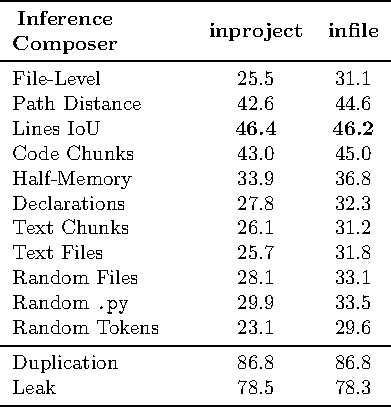
\includegraphics{tables/rq-a1.pdf}
    \shortcaption{Evaluation of DeepSeek-Coder-Base 1.3B}{Exact Match scores of DeepSeek-Coder-Base 1.3B benchmarked on the LCA}\label{tab:dseek-inference}
\end{table}

A noticeable difference is observed, allowing us to infer that the context provided to the model during inference has a significant impact on its performance. Some detailed findings are as follows:

\begin{enumerate}
\item In-context learning enables the model to leverage any form of meaningful context to improve \textit{infile} completion, indicating that API declarations are not the sole source of metric improvements and that project-level information provides auxiliary grounding for generation.
\item The Lines IoU approach proposes the most effective relevance function for retrieval-augmented generation among the presented methods, demonstrating that the model can achieve the same level of \textit{inproject} performance as \textit{infile}, given the context of sufficient quality.
\item The examination of Declarations indicates that function and class declarations alone do not provide a strong foundation for in-context learning capabilities; the functional code within their bodies is more important.
\item A comparison between Random \texttt{.py} and Text Files suggests that configuration and documentation files are less important for the model than randomly selected code examples in the context. The same observation applies to code comments and documentation strings produced by Text Chunks.
\item Even randomly selected files enhance the code completion capabilities of the model.
\item Random Tokens degrade performance only slightly compared to the File-Level composer, indicating that the model is highly, though not completely, robust to the presence of noisy context.
\item The model is capable of effectively copying (Duplication) and extracting (Leak) ground-truth lines from the context without requiring any additional training.
\end{enumerate}

\subsection{Fine-Tuning on Compositions}\label{sec:fine-tuning-on-compositions}

To estimate the impact of the context composition strategy employed during model fine-tuning, we subject the same model from the previous section to training with various composers. After fine-tuning, we benchmark the model to produce \tableref{tab:dseek-fine-tuning}.

\begin{table}[htbp]
    \centering
    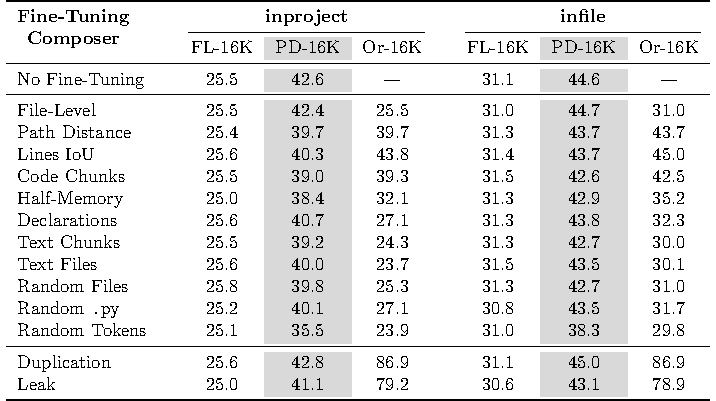
\includegraphics[width=\textwidth]{tables/rq-a2.pdf}
    \shortcaption{Evaluation of fine-tuned DeepSeek-Coder-Base 1.3B}{Exact Match scores of DeepSeek-Coder-Base 1.3B fine-tuned with different context composition strategies. The rows indicate the composer used to obtain the model checkpoint. The columns represent different evaluation setups: PD for Path Distance, FL for File-Level, and Or for the composer used during fine-tuning. All sequences are truncated to 16K tokens. The blank cells refer to the \tableref{tab:dseek-inference}.}\label{tab:dseek-fine-tuning}
\end{table}

The marginal differences in metric values suggest that this particular model is sufficiently trained and is not significantly affected by subsequent fine-tuning.

One might argue that the number of training steps is insufficient. To address this concern, we monitor the learning curves during training and observe that the metric improvements are too small to justify further scaling of this experimental direction. For instance, the best linear slope, \(1.28 \times 10^{-5}\) of EM, is achieved by the Lines IoU composer during the first \(512\) iterations. Applying a linear extrapolation of this slope implies that the model would require more iterations to gain 5 EM points than permitted by the learning rate scheduler. Furthermore, since the proxy metric for EM is cross-entropy loss, whose learning curves follow power-law scaling \parencite{kaplan2020}, this extrapolation remains extremely optimistic.

Additionally, we explored different setups to address the issue of the model's robustness to this type of fine-tuning. First, a different training dataset with lower data diversity was used earlier, which resulted in overfitting after the first epoch. Second, we experimented with other hyperparameter choices without success. Third, to eliminate researcher proficiency bias, the experiments were independently reproduced from scratch by another person, which is beyond the scope of this thesis.

\section{Out-of-Distribution Context Length}

In this section, we address the second pair of research questions: \hyperref[rq:rq-b1]{RQ.B1} and \hyperref[rq:rq-b2]{RQ.B2}. For both of them, we use OpenCoder-1.5B-Base and apply context window extension fine-tuning with sequences exceeding the original context window size of 4K tokens. The only exception is the File-Level composer, which we use to support our findings on the resource efficiency of repository-level pre-training under the in-distribution context length composer.

\subsection{Effect of Context Extension}\label{sec:effect-of-context-extension}

We assess the impact of repository-level pre-training on the previously obtained in-context learning capabilities of the model using the composition strategies accessible to OpenCoder-1.5B-Base, which has an original context size limitation of 4K tokens. The summarized results are presented in \tableref{tab:ocoder-in-context-retention}. For the extended version, which includes the effects observed with \textit{reversed} and \textit{irrelevant} order modifications, refer to \tableref{tab:ocoder-extension-extended}.

\begin{table}[htbp]
    \centering
    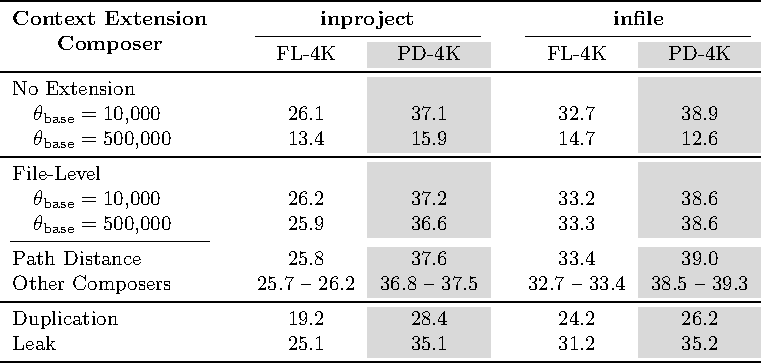
\includegraphics[width=\textwidth]{tables/rq-b1.pdf}
    \shortcaption{In-context learning capabilities of OpenCoder-1.5B-Base after context extension}{Exact Match scores of OpenCoder-1.5B-Base under different evaluation setups. The original model's performance is denoted by No Extension. The other rows represent the checkpoints obtained with the respective composers. Context extension is performed with 4K-token sequences for the File-Level and 16K-token sequences for all other composers. The column notations are consistent with the previous table.}\label{tab:ocoder-in-context-retention}
\end{table}

We draw three main observations from the table to address \hyperref[rq:rq-b1]{RQ.B1}:

\begin{enumerate}
\item ABF without additional fine-tuning significantly impairs the ICL capabilities.\newpage
\item The context extension procedure effectively restores model performance after RoPE frequency scaling. Even the File-Level composer, which utilizes input sequences up to 4K tokens, enables the model to adapt to the new \(\theta_{\mathrm{base}}\) value and maintain the same performance level as the original model.
\item Data leakage of ground-truth lines impedes the recovery of the model's ICL capabilities. This effect is particularly pronounced for the Duplication composer.
\end{enumerate}

\subsection[Influence of Composition on Context Extension]{Influence of Composition\\on Context Extension}\label{sec:influence-of-composition-on-context-extension}

In this section, we address the final research question \hyperref[rq:rq-b2]{RQ.B2} by evaluating the checkpoints obtained after context extension fine-tuning, using various composers to construct the training context. Our conclusions are drawn from \tableref{tab:ocoder-extension}, which is a subset of the comprehensive \tableref{tab:ocoder-extension-extended}.

\begin{table}[htbp]
    \centering
    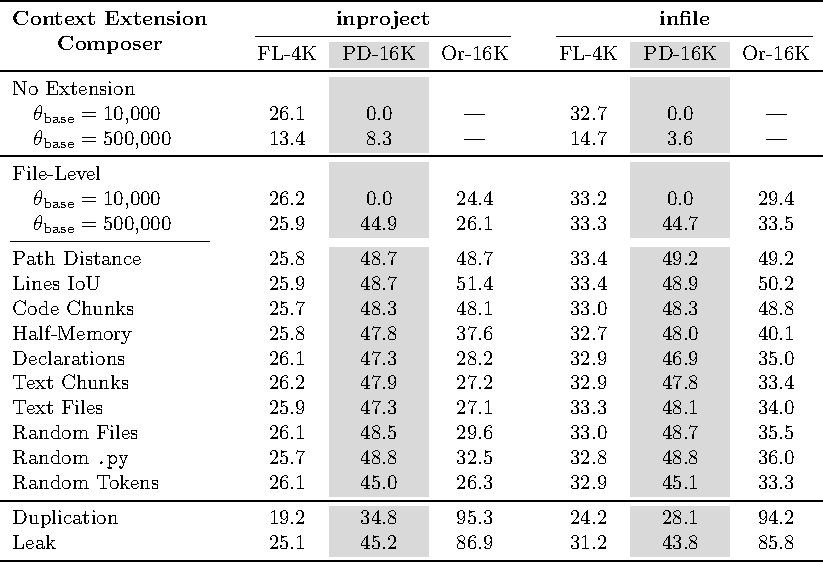
\includegraphics[width=\textwidth]{tables/rq-b2.pdf}
    \shortcaption{Evaluation of repository-level pre-trained OpenCoder-1.5B-Base}{Exact Match scores collected from the long-context evaluation of composer choices employed during the repository-level pre-training stage of OpenCoder-1.5B-Base. All clarifying remarks are consistent with the previous table. Blank cells indicate the absence of a repository-level pre-training stage in OpenCoder's development pipeline.}\label{tab:ocoder-extension}
\end{table}

\newpage
To summarize the outcomes of our study, we present the following observations:

\begin{enumerate}
\item As expected, the original model is unable to utilize the 16K context window. The preliminary base frequency adjustment provides only a negligible improvement and necessitates an additional optimization phase.
\item The context composition strategy employed during the repository-level pre-training stage has only a marginal impact on the final model quality. This finding suggests that adaptation to the RoPE adjustment is the primary driver of long-context improvements.
\item It is possible to significantly reduce computational requirements while still achieving competitive results at the repository-level pre-training stage. For instance, file-level training remains highly effective, even without any repository context and with a context window size limited to 4k tokens.
\item The Duplication composer proves its uncompetitiveness even when compared to the entirely irrelevant context obtained from Random Tokens. This suggests that the data must present at least some degree of challenge to the model in order to foster the development of additional capabilities.
\end{enumerate}

The main practical contribution of this research is the identification of a low-resource approach to repository-level pre-training. Context extension fine-tuning can be restricted to the Path Distance composer, requiring only 1B training tokens, while the File-Level presents an even more resource-efficient alternative, necessitating just 73M training tokens. We further demonstrate the utility of this setup by comparing it with DeepSeek-Coder-Base 1.3B, which used 8.4B tokens for repository-level pre-training, and Qwen2.5-Coder-1.5B~\parencite{hui2024}, which employed 300B tokens during the same stage. \figureref{fig:model-comparison} visualizes this comparison, and \figureref{fig:beyond-training-window-inproject} illustrates the performance scaling beyond the training context window for all four models.

\begin{figure}[ht]
    \centering
    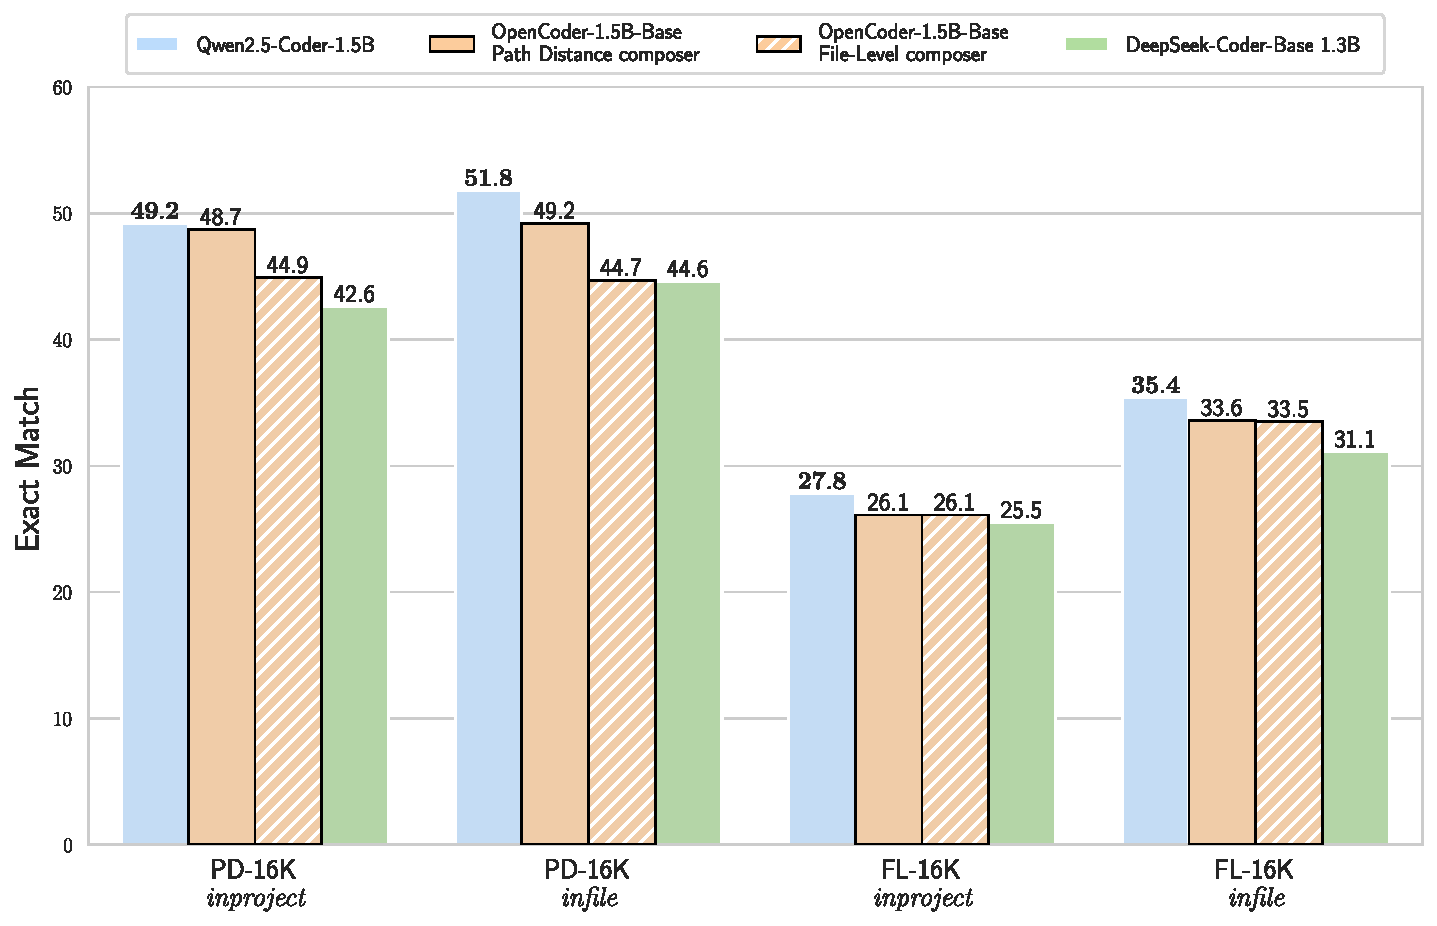
\includegraphics[width=\textwidth]{figures/model-comparison.pdf}
    \shortcaption{Comparison of two main checkpoints after context extention with Qwen2.5-Coder-1.5B and DeepSeek-Coder-Base-1.3B}{Comparison of our two main checkpoints with other existing Code LLMs of the same weight class. The PD-16K setup is used to produce the metric assessment.}\label{fig:model-comparison}
\end{figure}

\begin{figure}[ht]
    \centering
    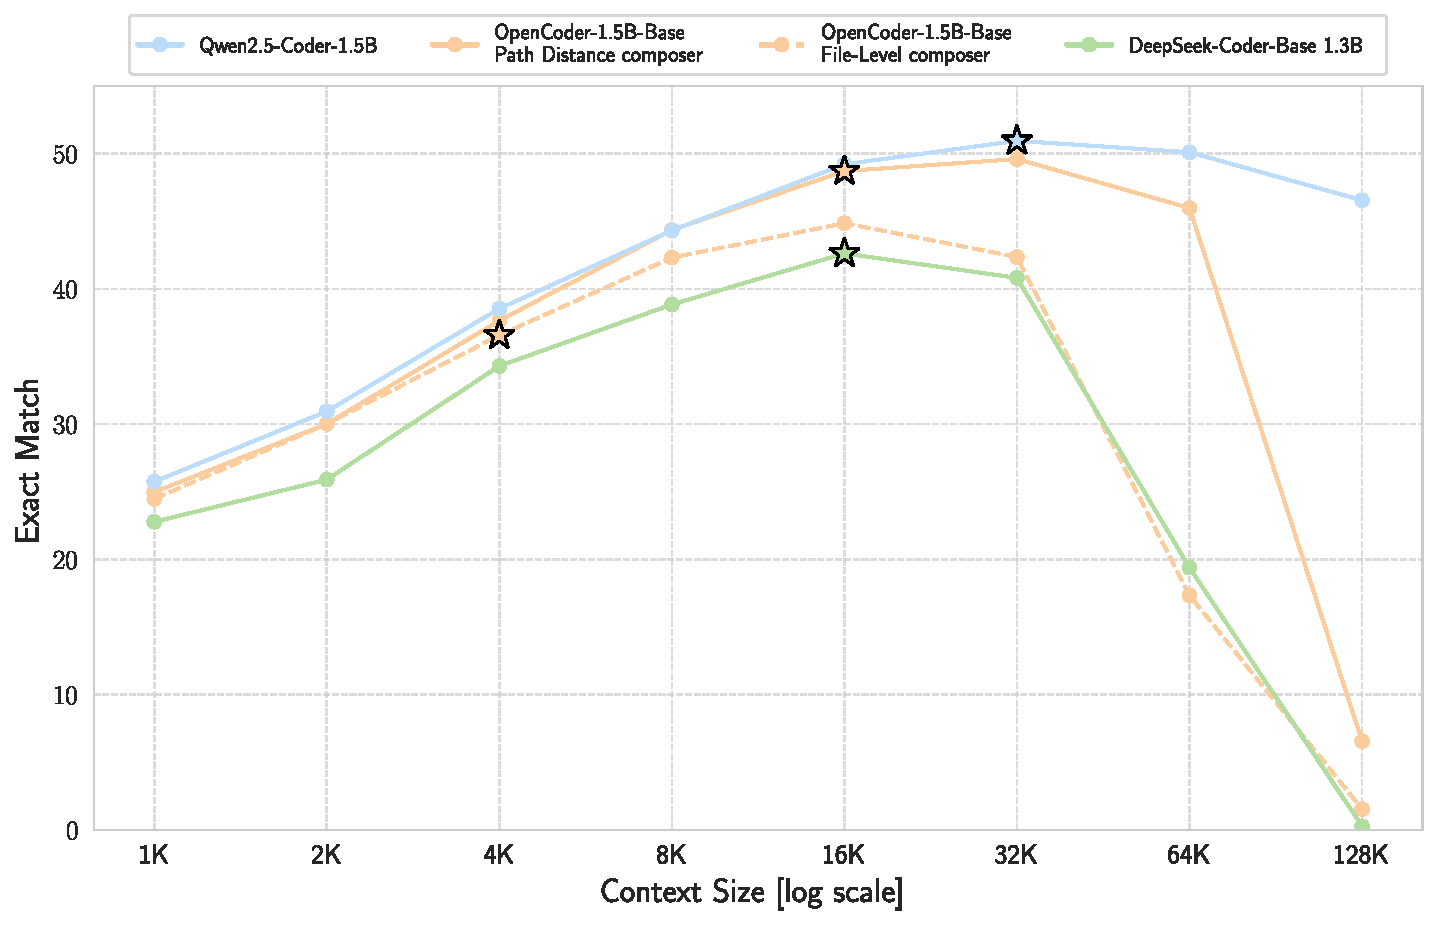
\includegraphics[width=\textwidth]{figures/beyond-training-window-inproject.pdf}
    \shortcaption{Performance scaling beyond context extension window (\textit{inproject})}{Evaluation of the performance scaling beyond the context extension window. The \textit{inproject} line type from the LCA benchmark is selected for visualization; the corresponding \figureref{fig:beyond-training-window-infile} presents results for the \textit{infile} category. ``1K'' refers to 1,024 tokens. The \raisebox{-0.3ex}{\FiveStarOpen} markers denote the context length used during repository-level pre-training stage.}\label{fig:beyond-training-window-inproject}
\end{figure}

We note that the same model's extrapolation behavior, as shown in \figureref{fig:beyond-training-window-inproject}, was partially reported by \citet{rozière2023}. Specifically, when the model is initialized with RoPE from scratch and trained on sequences up to \(N\) tokens, it is unable to extrapolate beyond its pre-training length. However, after applying ABF and optimizing for a few steps on sequences up to \(M > N\) tokens, the model learns to extrapolate not only beyond \(N\) tokens but also for values greater than \(M\). While we confirm this finding, the core novelty of our evaluation lies in the case where \(M = N\), which demonstrates the preservation of described properties.

\newpage
\section{Supplementary Results}

To diversify the research, in this section we provide a supplementary analysis of the experiments focused on investigating the effects of order modifications and gradient masking.

\subsection{Influence of Order Modifications}

The same conclusions regarding the preservation of ICL capabilities after the repository-level pre-training stage and the impact of composition on context extension apply to both the \textit{reversed} and \textit{irrelevant} order modifications. For example, although the checkpoint obtained with Lines IoU \textit{irrelevant} context extension during inference yields an EM score that is half that of its \textit{original} and \textit{reversed} counterparts, it achieves equivalent performance when the composer is switched to Path Distance. We attach \tableref{tab:ocoder-extension-extended} to present all metric values related to this observation.

\subsection{Gradient Masking}\label{sec:gradient-masking}

To avoid training on out-of-distribution lines, we consistently apply gradient masking to non-completion tokens when training with composers that produce distributions dissimilar to the completion file. Although this design choice is intuitive, the applicability of this technique to runs with inlier composers remains an open question.

To examine the impact of including all losses in the optimization process for the inlier composers, we conduct training runs both with and without masking. \tableref{tab:dseek-gradient-masking} shows the results of this experiment for the DeepSeek-Coder-Base 1.3B, and \tableref{tab:ocoder-gradient-masking} for the OpenCoder-1.5B-Base model. We then consider all these values except those for the Duplication composer to perform a one-sided paired t-test with the alternative hypothesis that the mean Exact Match of models trained with gradient masking is lower than that for full loss training. The reported \(p\)-value is \(1.9 \times 10^{-5}\), so we reject the null hypothesis at a significance level of \(\alpha = 0.05\). \figureref{fig:gradient-masking} visualizes the distribution of these metric differences.

\begin{figure}[ht]
    \centering
    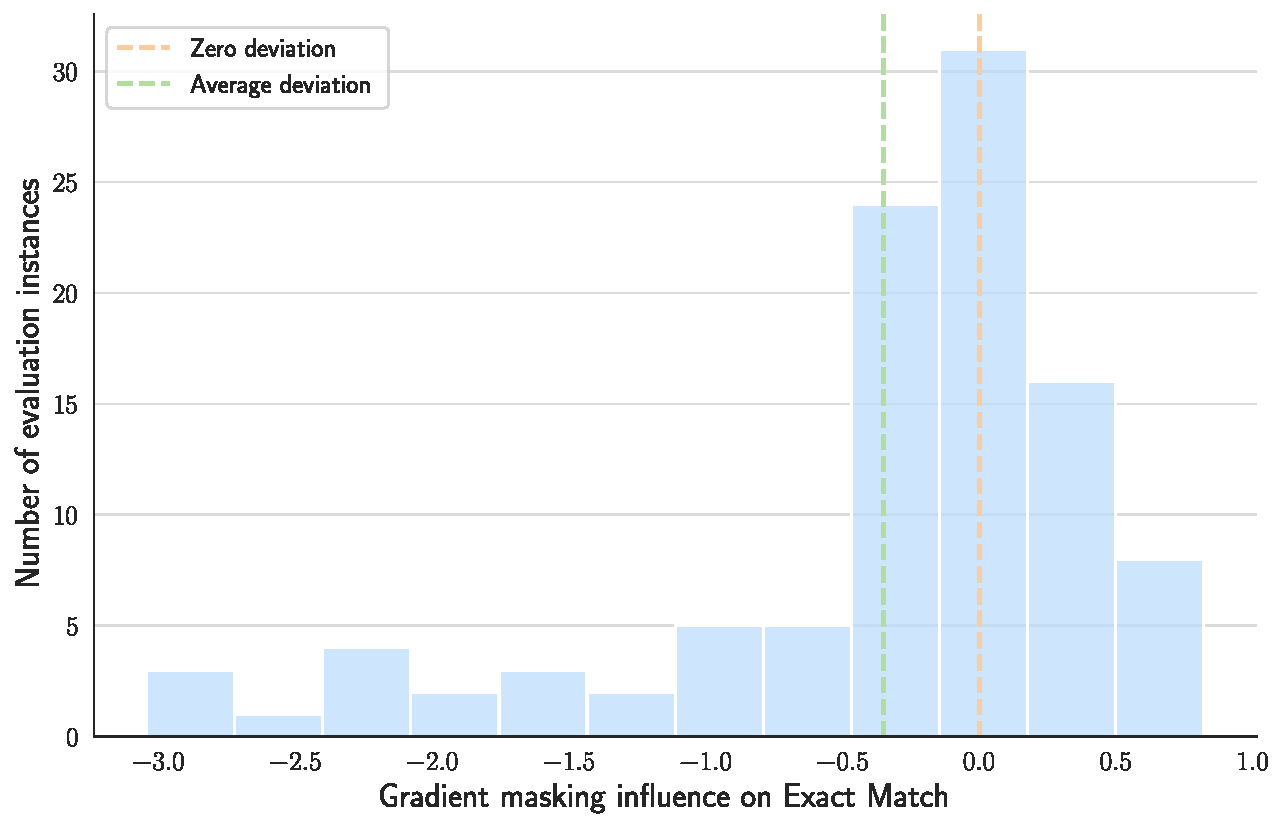
\includegraphics[width=\textwidth]{figures/gradient-masking.pdf}
    \shortcaption{Histogram of Exact Match score differences induced by gradient masking}{Histogram of the Exact Match differences between paired runs on inlier composers, with the Duplication composer excluded. Negative values indicate cases where gradient masking reduces model performance. The sample mean is \(-0.35\) EM points on a scale from \(-100\) to \(100\).}\label{fig:gradient-masking}
\end{figure}

Another observation is that disabling gradient masking eliminates the detrimental properties of the Duplication composer. We attribute this to the model being required to perform well on the first instance of the completion file presented in the context, which does not have access to the ground-truth lines to copy from.

\section{Limitations and Future Work}

\begin{sloppypar}
Although we have addressed all research questions and inferred various insights, several directions for scaling the conducted experiments and new prospects for extending the work further remain open.
\end{sloppypar}

The empirical results provided are based on the utilization of two Code LLMs, which narrows the generalizability of our research. This limitation is particularly pronounced for \hyperref[rq:rq-b1]{RQ.B1} and \hyperref[rq:rq-b2]{RQ.B2}, as OpenCoder is the only modern Code LLM released without repository-level pre-training, leaving no alternatives yet to scale this direction. We conclude that a better practice for model providers would be to release all major model checkpoints obtained throughout the development pipeline, as this would foster the growth of the field by outsourcing less compute-intensive exploration to the open research community.

The evidence of a repository-level pre-training setup that requires fewer resources and achieves competitive results suggests significant potential for future exploration of the optimal recipe for this stage. First, a mixed approach combining different composers to benefit from their individual factors can be explored. Second, other RoPE extension methods can be tested using the same\newpage\noindent experimental design. Third, a proper metric for token efficiency can be developed to assess the trade-off between the compute used and the performance achieved.

Another important line of future work is to verify the findings on other code-related tasks and test whether they can be transferred to the Natural Language Processing domain.
